\section{Data Crawler}

The data crawler is the smallest data processing unit within the data factory. The data crawler is evolved using a blue print of the R-A-P-T-O-R pipeline and bills-of-material consisting of code snippets and then spawn with an unique identity. Our data processing data crawlers is built to perform a single purpose and then made extinct once it completes the specific task.

\begin{figure}{!h}
    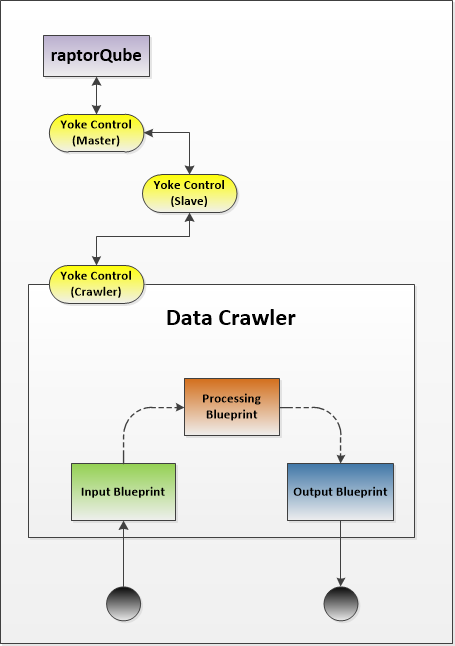
\includegraphics[width=3cm]{images/DataCrawler.png}
    \caption{Basic Data Crawler Blueprint.} \label{fig:datacrawler}
\end{figure}

The basic template for the data crawler (fig. \ref{fig:datacrawler}) is:

\begin{itemize}
    \item raptorQube - Core autonomous processing engine that controls the complete solution.
    \item Yoke Control (Master) - Master control yoke of data factory.
    \item Yoke Control (Slave) - Slave control yoke of data factory.
    \item Data Crawler - the crawler is the work cell for the processing.
    The crawler is evolve and spawn to perform a singular task in the processing workflow pipeline.
    The crawler consists of following to enable its dynamic processing.
    \begin{itemize}
        \item Yoke Control (Crawler)
        \item Input Blueprint
        \item Processing Blueprint
        \item Output Blueprint
    \end{itemize}
\end{itemize}

The factory supports the following types of crawlers:
\begin{itemize}
    \item Rapid Assimilator - crawler builds the ecosystem for each factory.
    \item Scout - crawler scouts for new or changed data entities in the ecosystem for each factory.
    \item Explorer - crawler explores any entities found by scout.
    \item Builder - crawler builds the processing pipeline for the R-A-P-T-O-R engine in the ecosystem for each factory.
    \item Monitor - crawler monitors the ecosystem to collect information about each factory's ecosystem.
\end{itemize}

